
\documentclass{beamer}
\usecolortheme{dove}
\setbeamertemplate{navigation symbols}{}
\usepackage{amsmath,amssymb,amsfonts,amsthm, multicol, subfigure, color}
\usepackage{bm}
\usepackage{graphicx}
\usepackage{tabularx}
\usepackage{booktabs}
\usepackage{hyperref}
\usepackage{pdfpages}
\usepackage{xcolor}
\definecolor{seagreen}{RGB}{46, 139, 87}
\def\independenT#1#2{\mathrel{\rlap{$#1#2$}\mkern2mu{#1#2}}}
\newcommand\indep{\protect\mathpalette{\protect\independenT}{\perp}}
\def\log{\text{log}}
\newcommand\logit{\text{logit}}
\newcommand\iid{\stackrel{\text{iid}}{\sim}}
\newcommand\E{\text{E}}
\newcommand\V{\text{V}}
\renewcommand\P{\text{P}}
\newcommand{\Cov}{\text{Cov}}
\newcommand{\Cor}{\text{Cor}}
\newcommand\doop{\texttt{do}}
\usepackage{stackrel}
\usepackage{tikz}
\usetikzlibrary{arrows,shapes.arrows,positioning,shapes,patterns,calc}
\newcommand\slideref[1]{\vskip .1cm \tiny \textcolor{gray}{{#1}}}
\newcommand\red[1]{\color{red}#1}
\newcommand\blue[1]{\color{blue}#1}
\newcommand\gray[1]{\color{gray}#1}
\newcommand\seagreen[1]{\color{seagreen}#1}
\newcommand\purple[1]{\color{purple}#1}
\newcommand\orange[1]{\color{orange}#1}
\newcommand\black[1]{\color{black}#1}
\newcommand\white[1]{\color{white}#1}
\newcommand\teal[1]{\color{teal}#1}
\newcommand\magenta[1]{\color{magenta}#1}
\newcommand\Fuchsia[1]{\color{Fuchsia}#1}
\newcommand\BlueGreen[1]{\color{BlueGreen}#1}
\newcommand\bblue[1]{\textcolor{blue}{\textbf{#1}}}
\newcommand\bred[1]{\textcolor{red}{\textbf{#1}}}
\newcommand\bgray[1]{\textcolor{gray}{\textbf{#1}}}
\newcommand\bgreen[1]{\textcolor{seagreen}{\textbf{#1}}}
\newcommand\bref[2]{\href{#1}{\color{blue}{#2}}}
\colorlet{lightgray}{gray!40}
\pgfdeclarelayer{bg}    % declare background layer for tikz
\pgfsetlayers{bg,main} % order layers for tikz
\newcommand\mycite[1]{\begin{scriptsize}\textcolor{darkgray}{(#1)}\end{scriptsize}}
\newcommand{\tcframe}{\frame{
%\small{
\only<1|handout:0>{\tableofcontents}
\only<2|handout:1>{\tableofcontents[currentsection]}}
%}
}

\usepackage[round]{natbib}
\bibliographystyle{humannat-mod}
\setbeamertemplate{enumerate items}[default]
\usepackage{mathtools}

\newcommand{\goalsframe}{\begin{frame}{Learning goals for today}
At the end of class, you will be able to:
\begin{enumerate}
\item Understand DAGs more fully
\begin{itemize}
\item DAGs are nonparametric
\item DAGs are hard to learn from data
\end{itemize}
\item Generalize from a sample to a population
\begin{itemize}
\item Encode sampling assumptions in DAGs
\end{itemize}
\end{enumerate} \vskip .2in
\end{frame}}

\title{6. Population inference from samples}
\author{Ian Lundberg\\Cornell Info 6751: Causal Inference in Observational Settings\\Fall 2022}
\date{8 Sep 2022}

\begin{document}

\maketitle

\begin{frame}{Comments on Problem Set 1}

Definition of potential outcomes
\begin{itemize}
\item $\{Y_i^1,Y_i^0\}$ are potential outcomes.\\When $A_i = 1$, then $Y_i^1$ is factual and $Y_i^0$ is counterfactual.\\When $A_i = 0$, then these are reversed.\\This is why potential, not necessarily counterfactual.
\item $Y^a$ is the outcome of a randomly sampled unit assigned to treatment value $a$. In itself, it is not an average over a group---that would be $\E(Y^a)$.
\end{itemize}

\end{frame}


\begin{frame}{Comments on Problem Set 1}

$\E(Y\mid A = 1)> \E(Y\mid A = 0)$
\begin{itemize}
\item Descriptive
\item Outcomes were higher, on average, for those who got the treatment 
\end{itemize} \vskip .2in

$\E(Y^1)> \E(Y^0)$
\begin{itemize}
\item Causal 
\item The treatment (1 vs 0) increases outcomes, on average
\end{itemize} \vskip .2in

$Y_i^1 > Y_i^0$ for all $i$
\begin{itemize}
\item Causal 
\item The treatment (1 vs 0) increases the outcome for every unit
\end{itemize}

\end{frame}

\begin{frame}{Comments on Problem Set 1}
\begin{center}
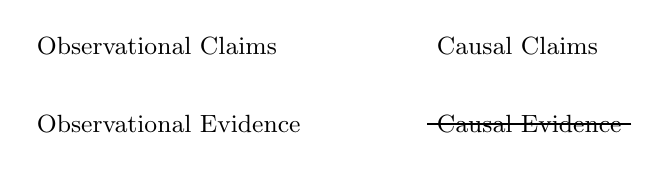
\begin{tikzpicture}[x = 2in]
\node[font = \small, anchor = west] at (1,1) {Observational Claims};
\node[font = \small, anchor = west] at (1,0) {Observational Evidence};
\node[font = \small, anchor = west] at (2,1) {Causal Claims};
\node[font = \small, anchor = west] (wrong) at (2,0) {Causal Evidence};
\draw<2->[thick] (wrong.east) -- (wrong.west);
\end{tikzpicture}
\end{center} \vskip .2in
\onslide<3->{``...all causal inference is based on assumptions that cannot be derived from observations alone,'' (Greenland, Pearl, \& Robins 1999, p. 47)} \vskip .2in
\onslide<4->{There is no causal evidence.\\There is only observational evidence,\\which speaks to causal claims under assumptions.}
\end{frame}


\goalsframe

\begin{frame}[t]{DAGs are nonparametric}
\pause

\begin{center}
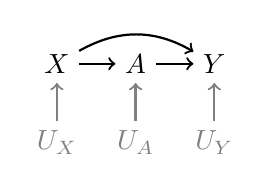
\begin{tikzpicture}
\node (x) at (-1,0) {$X$};
\node (a) at (0,0) {$A$};
\node (y) at (1,0) {$Y$};
\draw[->, thick] (x) -- (a);
\draw[->, thick] (a) -- (y);
\draw[->, thick] (x) to[bend left] (y);
\onslide<5->{
\node[gray] (ux) at (-1,-1) {$U_X$};
\node[gray] (ua) at (0,-1) {$U_A$};
\node[gray] (uy) at (1,-1) {$U_Y$};
\draw[->, thick, gray] (ux) -- (x);
\draw[->, thick, gray] (ua) -- (a);
\draw[->, thick, gray] (uy) -- (y);
}
\end{tikzpicture}
\end{center}
\onslide<3->{
This does \bred{not} mean
$$Y = \beta_0 + \beta_1 X + \beta_2 A + \epsilon$$
} \vspace{-.3in}

\onslide<4->{
This \bgreen{does} mean
\begin{itemize}
\item $A = f(X, U_A)$ for some function $f()$
\item $Y = g(X,A,U_Y)$ for some function $g()$
\end{itemize}
}
\onslide<6->{
which allows that
\begin{itemize}
\item The effect of $A$ may depend on $X$ (heterogeneity)
\item $\E(Y\mid X, A)$ may be a nonlinear function of each input
\end{itemize}
}

\end{frame}

\begin{frame}[t]{DAGs are nonparametric: Why this is really great}
\begin{center}
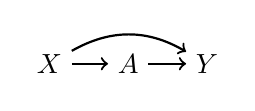
\begin{tikzpicture}
\node (x) at (-1,0) {$X$};
\node (a) at (0,0) {$A$};
\node (y) at (1,0) {$Y$};
\draw[->, thick] (x) -- (a);
\draw[->, thick] (a) -- (y);
\draw[->, thick] (x) to[bend left] (y);
\end{tikzpicture} \pause
\end{center}
This tells us:
$$\underbrace{\E(Y^a\mid X = x)}_\text{Causal Quantity} = \underbrace{\E(Y\mid A = a, X = x)}_\text{Statistical Quantity}$$ \pause
Left statement:
\begin{itemize}
\item Among everyone with $X = x$,
\item the average outcome if we set $A = a$
\end{itemize} \vskip .2in \pause

Right statement:
\begin{itemize}
\item Among everyone with $X = x$ and $A = a$,
\item the average outcome
\end{itemize}\vskip .1in
\begin{center} \pause
These are two \bblue{different sets} of people \large
\end{center}
\end{frame} 

\begin{frame}[t]{DAGs are nonparametric: Why this is really great}
\begin{center}
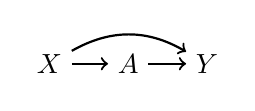
\begin{tikzpicture}
\node (x) at (-1,0) {$X$};
\node (a) at (0,0) {$A$};
\node (y) at (1,0) {$Y$};
\draw[->, thick] (x) -- (a);
\draw[->, thick] (a) -- (y);
\draw[->, thick] (x) to[bend left] (y);
\end{tikzpicture}
\end{center}
This tells us:
$$\underbrace{\E(Y^a\mid X = x)}_\text{Causal Quantity} = \underbrace{\E(Y\mid A = a, X = x)}_\text{Statistical Quantity}$$ \pause
Once the DAG gives us the above,\\ \pause
we can use \bblue{any} prediction function\\ \pause
for the statistical part.
\end{frame} 

\begin{frame}[t]{DAGs are nonparametric: Why this is really great}
\begin{center}
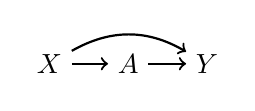
\begin{tikzpicture}
\node (x) at (-1,0) {$X$};
\node (a) at (0,0) {$A$};
\node (y) at (1,0) {$Y$};
\draw[->, thick] (x) -- (a);
\draw[->, thick] (a) -- (y);
\draw[->, thick] (x) to[bend left] (y);
\end{tikzpicture}
\end{center}
This contrasts with standard econometrics \pause
$$Y = \alpha + \beta_1X + \gamma A + \eta XA + \epsilon$$ \pause
\begin{itemize}
\item $\{\beta,\gamma\}$ are ``main effects'' \pause
\item $\eta$ is an ``interaction'': the effect of $A$ varies by $X$ \pause
\item Key assumption: $A\indep\epsilon$, or $A$ is ``exogenous''
\end{itemize} 
That requires us to do \bblue{both} causal reasoning \bblue{and}\\statistical reasoning simultaneously. \vskip .2in
DAGs support causal reasoning \bblue{before} statistical reasoning
\end{frame} 

\begin{frame}[t]{DAGs are nonparametric: Why this is really great}
\begin{center}
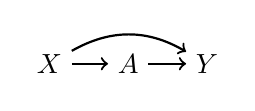
\begin{tikzpicture}
\node (x) at (-1,0) {$X$};
\node (a) at (0,0) {$A$};
\node (y) at (1,0) {$Y$};
\draw[->, thick] (x) -- (a);
\draw[->, thick] (a) -- (y);
\draw[->, thick] (x) to[bend left] (y);
\end{tikzpicture}
\end{center}
$$\underbrace{\E(Y^a\mid X = x)}_\text{Causal Quantity} = \underbrace{\E(Y\mid A = a, X = x)}_\text{Statistical Quantity}$$ \vskip .3in
Let's pause to discuss this.

\end{frame}

\goalsframe

\begin{frame}{Causal Discovery\footnote{\tiny See Spirtes, P., Glymour, C. N., Scheines, R., \& Heckerman, D. (2000). Causation, Prediction, and Search. MIT Press.}: DAGs are hard to learn from data} \pause
\begin{center}
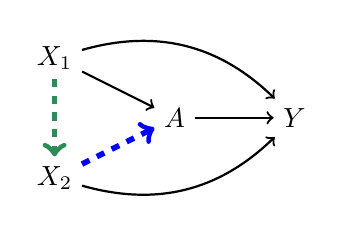
\begin{tikzpicture}[y = .3in, x = .6in]
\node (x1) at (-1,1) {$X_1$};
\node (x2) at (-1,-1) {$X_2$};
\node (a) at (0,0) {$A$};
\node (y) at (1,0) {$Y$};
\draw[->, thick] (x1) -- (a);
\draw[->, thick] (a) -- (y);
\draw[->, thick] (x1) to[bend left] (y);
\draw[->, thick] (x2) to[bend right] (y);
\draw<3->[->, line width = 2pt, dashed, blue] (x2) -- (a);
\draw<3->[->, line width = 2pt, dashed, seagreen] (x1) -- (x2);
\end{tikzpicture}
\end{center} \pause \pause
Can data tell us whether the dashed edges exist? \vskip .2in

\pause
\begin{itemize}
\item In the absence of both edges, \pause $X_1\indep X_2$ and $X_2\indep A$ \pause
\item In the absence of the blue edge, \pause $X_2\indep A\mid X_1$ \pause
\item In the absence of the green edge, \pause $X_1\indep X_2$ and $X_1\not\indep X_2\mid A$
\end{itemize}
\end{frame}

\begin{frame}{Causal Discovery\footnote{\tiny See Spirtes, P., Glymour, C. N., Scheines, R., \& Heckerman, D. (2000). Causation, Prediction, and Search. MIT Press.}: DAGs are hard to learn from data}
Will data replace human researchers? \vskip .2in \pause
I think not. \vskip .2in \pause
Often, what we want to know cannot be answered by the data. \vskip .2in \pause
Example: Does the unobserved $U$ confound treatment assignment?
\begin{center}
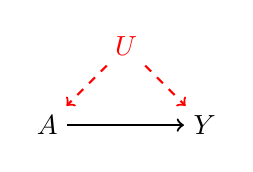
\begin{tikzpicture}
\node (a) at (0,0) {$A$};
\node (y) at (2,0) {$Y$};
\node[red] (u) at (1,1) {$U$};
\draw[->, thick] (a) -- (y);
\draw[->, thick, red, dashed] (u) -- (a);
\draw[->, thick, red, dashed] (u) -- (y);
\end{tikzpicture}
\end{center} \pause \vskip .1in
$A$ and $Y$ are associated either way.\\\pause The absence of $U$ is a completely untestable assumption.
\end{frame}

\begin{frame}

As a general rule, the DAG encodes\\\bblue{substantive theory} (made by a human)\vskip .2in rather than \bgreen{data} (crunched by a computer)
\end{frame}

\begin{frame}{Some academic history of DAGs}
\begin{itemize}
	\item Historical roots in path models in the 1920s
	\begin{itemize}
		\item Wright, S. (1921). Correlation and causation. Part I: Method of path coefficients. Journal of Agricultural Research, 20(7), 557-585.
	\end{itemize}
	\item Linear path models in the 1960s
	\begin{itemize}
		\item Duncan, O. D. (1966). Path analysis: Sociological examples. American Journal of Sociology, 72(1), 1-16.
	\end{itemize}
	\item Landmark contributions: Pearl, Greenland, Robins
	\begin{itemize}
		\item \bblue{(assigned)} Greenland, S., Pearl, J., \& Robins, J. M. (1999). Causal diagrams for epidemiologic research. Epidemiology, 37-48.
		\item Pearl, J. (2000). Causality. Cambridge University Press.
		\item Pearl, J., \& Mackenzie, D. (2018). The Book of Why: The New Science of Cause and Effect. Basic Books.
	\end{itemize}
	\item More accessible introduction for social scientists
	\begin{itemize}
		\item Morgan, S. L., \& Winship, C. (2015). Counterfactuals and Causal Inference. Cambridge University Press.
	\end{itemize}
\end{itemize}
\end{frame}

\goalsframe

\begin{frame}

\huge Sample $\rightarrow$ Population

\end{frame}

\begin{frame}{Fun example}

\only<1>{
Wang, Rothschild, Goel, \& Gelman\vskip .2in
Survey of \bblue{Xbox users} to forecast the 2012 election!\footnote{Wang, W., Rothschild, D., Goel, S., \& Gelman, A. (2015). \bref{https://doi.org/10.1016/j.ijforecast.2014.06.001}{Forecasting elections with non-representative polls.} International Journal of Forecasting, 31(3), 980-991.}
}
\includegraphics<2>[width = \textwidth]{figures/wangFig1}
\includegraphics<3>[width = \textwidth]{figures/wangFig3}

\end{frame}

\begin{frame}
Today we will formalize the conditions under which this works
\end{frame}

\begin{frame}[t] \vskip .2in
Imagine a study:\pause
\begin{itemize}
\item We randomly sample 1,000 voters from the U.S. voter file. \pause
\item We pay them \bblue{whatever it takes} \pause
\item \bblue{100\%} respond. \pause
\item We ask them a question: \pause
\begin{itemize}
\item Was Barack Obama the best president\\of the past 20 years?
\end{itemize}
\end{itemize} \pause
Can we draw conclusions about the population of U.S. voters? \vskip .3in \pause
{\Large Yes! A probability sample}
\end{frame}

\begin{frame}[t] \vskip .2in
Imagine another study:\pause
\begin{itemize}
\item We randomly sample 1,000 voters from the U.S. voter file. \pause
\item We pay them \bblue{\$500} to participate.
\item Only \bblue{90\%} respond. \pause
\item We ask them a question:
\begin{itemize}
\item Was Barack Obama the best president\\of the past 20 years?
\end{itemize}
\end{itemize} \pause
Can we draw conclusions about the population of U.S. voters?\vskip .3in \pause
{\Large Iffy. Almost a probability sample}
\end{frame}

\begin{frame}[t] \vskip .2in
Imagine another study:
\begin{itemize}
\item We randomly sample 1,000 voters from the U.S. voter file.
\item We can only pay them \bblue{\$5} to participate.
\item Only \bblue{10\%} respond.
\item We ask them a question:
\begin{itemize}
\item Was Barack Obama the best president\\of the past 20 years?
\end{itemize}
\end{itemize}
Can we draw conclusions about the population of U.S. voters? \pause \vskip .2in
{\Large Big worry:\vskip .1in Do we believe that selection into the sample\\is independent of Obama support?}
\end{frame}

\begin{frame}
\begin{center}
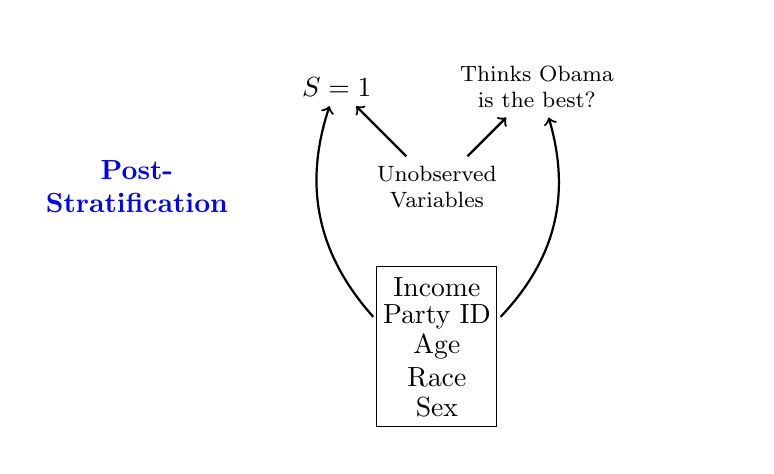
\begin{tikzpicture}[x = .5in, y = .5in]
\node at (-4,-3.5) {};
\node at (3,.5) {};
\node (s) at (-1,0) {$S = 1$};
\node<2->[align = center, font = \footnotesize] (y) at (1,0) {Thinks Obama\\is the best?};
\node<3-11>[align = center, font = \footnotesize] (u) at (0,-1) {Unobserved\\Variables};
\draw<3-11>[->, thick] (u) -- (y);
\draw<4-11>[->, thick] (u) -- (s);
%\draw<12>[->, thick, dashed] (u) -- (y);
%\draw<12>[->, thick, dashed] (u) -- (s);
\node<5-> (income) at (0,-2) {Income};
\node<6-> (party) at (0,-2.3) {Party ID};
\node<7-> (age) at (0,-2.6) {Age};
\node<8-> (race) at (0,-2.9) {Race};
\node<9-> (sex) at (0,-3.2) {Sex};
\draw<10->[->, thick] (party.west) to[bend left] (s);
\draw<11->[->, thick] (party.east) to[bend right] (y);
\draw<13-> (-.6,-3.4) rectangle (.6,.-1.8);
\node<19>[align = center] at (-3,-1) {\bblue{Post-}\\\bblue{Stratification}};
\end{tikzpicture}
\end{center} \vspace{-.3in}
\onslide<14->{If this is the case:}
\begin{enumerate}
\item<15-> Split into sample subgroups \hfill (in sample)
\item<16-> Take the mean Obama support \hfill (in sample)
\item<17-> Find each subgroup size in all voter records \hfill (in population)
\item<18-> Average over subgroups, weighted by the population size \hfill (population estimate!)
\end{enumerate}
\end{frame}

\begin{frame}

A step further: No probability sample. \vskip .2in \pause
We sample random passers-by on the streets of Chicago. \vskip .2in \pause
\begin{itemize}
\item Was Barack Obama the best president\\of the past 20 years?
\end{itemize}

\end{frame}

\begin{frame}
\begin{center}
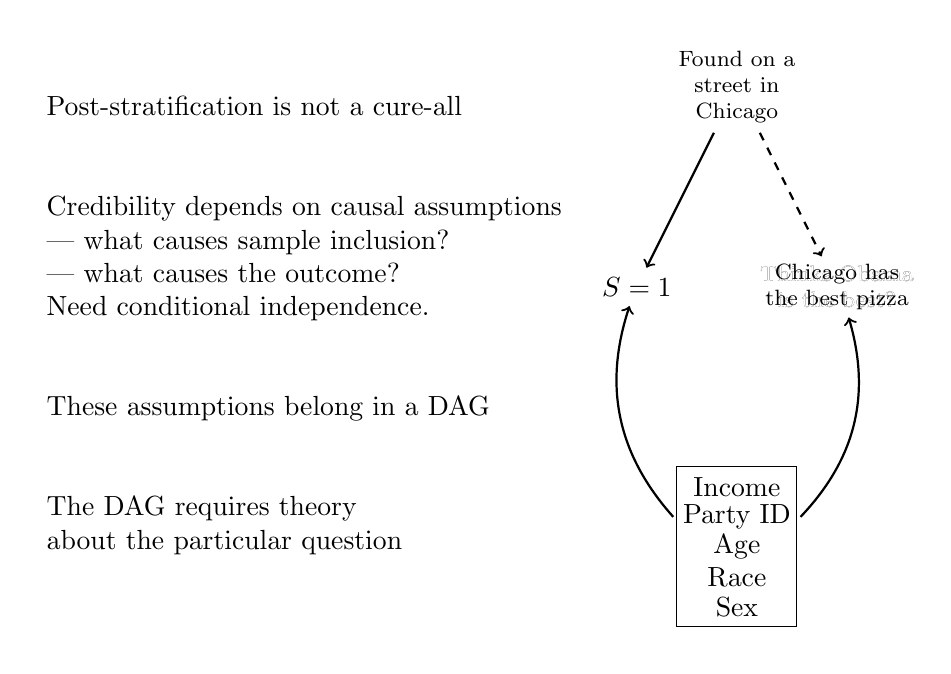
\begin{tikzpicture}[x = .5in, y = .5in]
\node at (-7,-3.5) {};
\node at (0,2.5) {};
\node<4->[anchor = north west, align = left] at (-7,2) {Post-stratification is not a cure-all};
\node<5->[anchor = north west, align = left] at (-7,1) {Credibility depends on causal assumptions\\--- what causes sample inclusion?\\--- what causes the outcome?\\Need conditional independence.};
\node<6->[anchor = north west, align = left] at (-7,-1) {These assumptions belong in a DAG};
\node<8->[anchor = north west, align = left] at (-7,-2) {The DAG requires theory\\about the particular question};
\node (s) at (-1,0) {$S = 1$};
\node<1-6>[align = center, font = \footnotesize] (y) at (1,0) {Thinks Obama\\is the best?};
\node<7->[align = center, font = \footnotesize, white] (y) at (1,0) {Thinks Obama\\is the best?};
\node<7->[align = center, font = \footnotesize] at (1,0) {Chicago has\\the best pizza};
\node (income) at (0,-2) {Income};
\node (party) at (0,-2.3) {Party ID};
\node (age) at (0,-2.6) {Age};
\node (race) at (0,-2.9) {Race};
\node (sex) at (0,-3.2) {Sex};
\draw[->, thick] (party.west) to[bend left] (s);
\draw[->, thick] (party.east) to[bend right] (y);
\draw (-.6,-3.4) rectangle (.6,.-1.8);
\node<2->[align = center, font = \footnotesize] (u) at (0,2) {Found on a\\street in\\Chicago};
\draw<2->[->, thick] (u) -- (s);
\draw<3->[->, thick, dashed] (u) -- (y);
\end{tikzpicture}
\end{center}
\end{frame}

\begin{frame}{Westreich et al. 2019} \pause

We often care about \bgreen{internal validity} \pause
\begin{itemize}
\item Have I identified the causal effect well in my sample?
\end{itemize} \pause
and also about \bgreen{external validity}
\begin{itemize} \pause
\item Does my sample speak to the population of interest?
\end{itemize} \pause
The authors combine these to discuss \bblue{target validity}

\end{frame}

\begin{frame}{Westreich et al. 2019, Fig 1 (modified)}
\scalebox{1.3}{
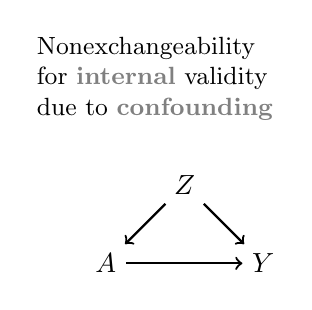
\begin{tikzpicture}
\node[anchor = north west, font = \small, align = left] at (-1,3) {Nonexchangeability\\for \bgray{internal} validity\\due to \bgray{confounding}};
\node (a) at (0,0) {$A$};
\node (y) at (2,0) {$Y$};
\node (z) at (1,1) {$Z$};
\draw[->, thick] (a) -- (y);
\draw[->, thick] (z) -- (a);
\draw[->, thick] (z) -- (y);
\end{tikzpicture} \qquad
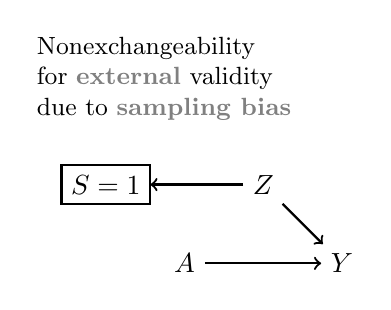
\begin{tikzpicture}
\node[anchor = north west, font = \small, align = left] at (-2,3) {Nonexchangeability\\for \bgray{external} validity\\due to \bgray{sampling bias}};
\node (a) at (0,0) {$A$};
\node (y) at (2,0) {$Y$};
\node (z) at (1,1) {$Z$};
\node (s) at (-1,1) {$S = 1$};
\draw[thick] (s.south west) rectangle (s.north east);
\draw[->, thick] (a) -- (y);
\draw[->, thick] (z) -- (y);
\draw[->, thick] (z) -- (s);
\end{tikzpicture}}
\end{frame}

\goalsframe

\begin{frame}{Let me know what you are thinking}

\begin{huge} \bref{https://tinyurl.com/CausalQuestions}{tinyurl.com/CausalQuestions} \end{huge}
\vskip .7in

Office hours TTh 11am-12pm and at \bref{https://calendly.com/ianlundberg/office-hours}{calendly.com/ianlundberg/office-hours}\\Come say hi!

\end{frame}

\end{document}

